%% tags: [breadth first search]
%% source: 2023-sp-redemption_midterm_02
\begin{prob}
    Suppose a BFS is run on the graph below using node 1 as the source node. Which
    node will be the BFS predecessor of node 8? You should use the convention that neighbors
    are produced in ascending order by label.

    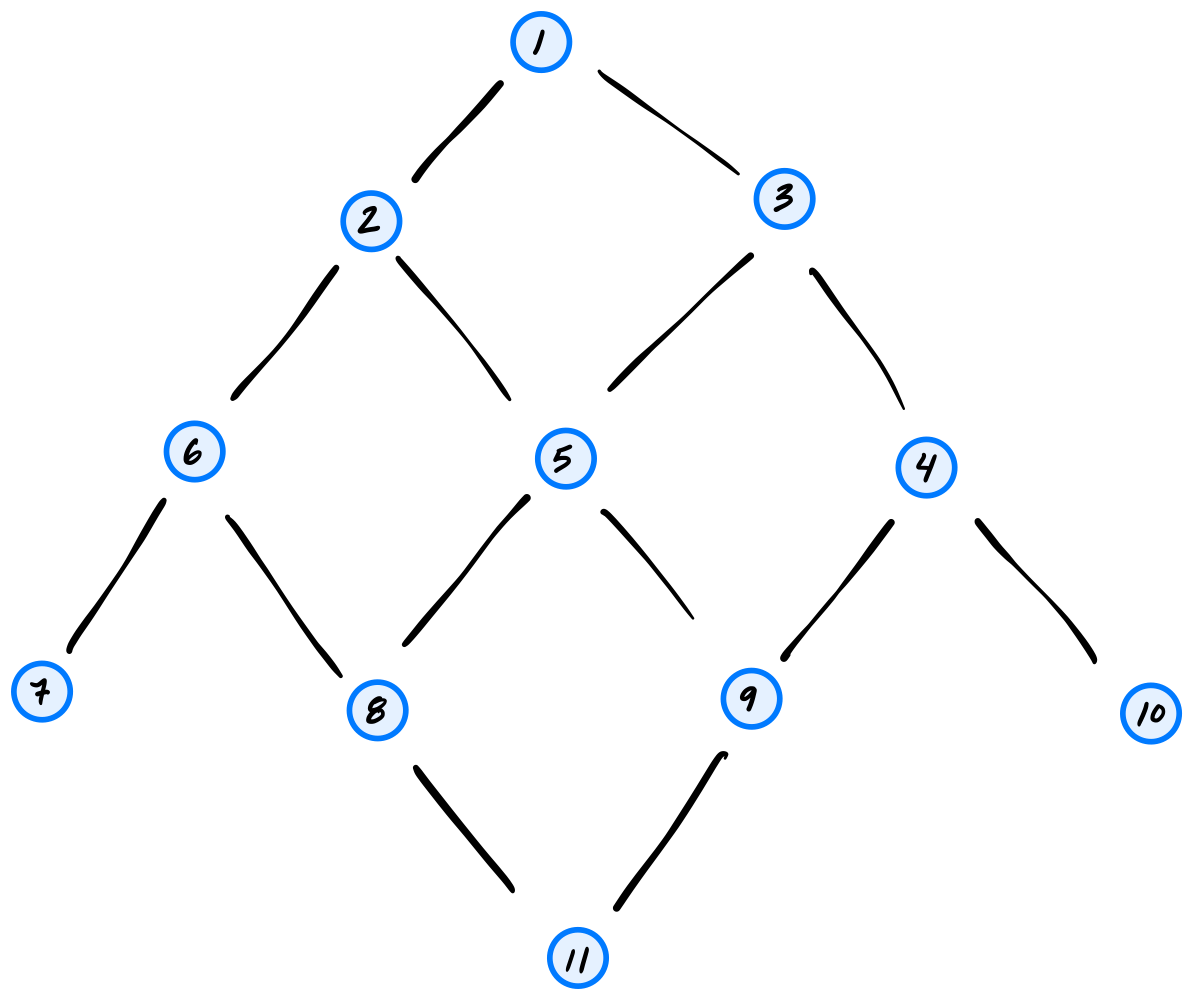
\includegraphics[width=.6\textwidth]{./fig/g2.png}

    \begin{soln}
        5
    \end{soln}

\end{prob}
